% GENERAL INFORMATION: HardwareX is an open access journal established to promote free and open source designing, building and customizing of scientific infrastructure (hardware). For more details on best practices for sharing open hardware see http://www.oshwa.org/sharing-best-practices/

\documentclass[11pt, letterpaper]{article}
\usepackage[utf8]{inputenc}
\usepackage[margin=1.5cm]{geometry} % Default 1.5cm, For review 2cm?
\usepackage{titlesec}
\usepackage{tabu}
\usepackage{enumitem}
\usepackage{amssymb}
\usepackage{xcolor}
\usepackage{verbatim}
\usepackage{graphicx}
\usepackage{setspace}
\usepackage{lineno}
\usepackage{makecell}
\newlist{selectlist}{itemize}{2}
\setlist[selectlist]{label=$\square$,leftmargin=*,noitemsep,topsep=0pt}

\usepackage{lmodern}

\usepackage{hyperref}
\hypersetup{
    colorlinks=true,
    linkcolor=blue,
    filecolor=magenta,      
    urlcolor=blue,
    citecolor={blue},
}
 
\urlstyle{same}

% Set up the section label formatting
\titleformat{\section}[block]{\hspace{1em}\bfseries}{\thesection.}{0.5em}{} 
\titleformat{\subsection}[block]{\hspace{1em}}{\thesubsection}{0.5em}{}

% Settings for Review
%\doublespacing
%\linenumbers

\begin{document}
% Create the title block
\begin{flushleft}


% Remove all text in italics when filling out the template and replace with your manuscripts corresponding text in regular font.
%\textit{Text in italics are template instructions. Remove and replace all instructions with regular font text.}

\setlength{\parindent}{0pt}
\setlength{\parskip}{10pt}
% \textbf{\large HardwareX article template}


%
% Background Information
%
%Insert title
%Max. 20 words. A good title should contain the fewest possible words that adequately describe the content of a paper.
\textbf{Title} \\
PolyWAG: Autonomous filtered water sampling for eDNA 
%\textit{Please avoid acronyms and abbreviations where possible.}

%
% Insert Authors
%
\textbf{Authors} \\
Kai Roy * Riley Prince * Marc Belinga * John Selker * Chet Udell
% List all authors. Please mark the corresponding author with (*)

%
% Insert Affiliations
%
\textbf{Affiliations} \\ 
OPEnS Lab, Oregon State University, Corvallis, OR, United States
%\textit{Please include the full address of each author institution}


%
% Insert Contact Email
%
% > Include institutional email address of the corresponding author
% > Institutional email address preferred. If you have a Twitter handle, please add it here ‘twitter: \@....’
\textbf{Corresponding author’s email address and Twitter handle}\\ 
Kai Roy - kaikurisakaroy\@gmail.com \\
Riley Prince - princeri@oregonstate.edu \\
Marc Belinga -  \\
John Selker - john.selker@oregonstate.edu \\
Chet Udell - udellc@oregonstate.edu


%
% Insert Abstract
%
% > Max. 200 words. 
% > Remember that the abstract is what readers see first in electronic abstracting and indexing services. 
% > This is the advertisement of your article. Make it interesting, and easy to be understood. 
% > Be accurate and specific, keep it as brief as possible.
\textbf{Abstract} \\ 
Environmental DNA (eDNA) is an ideal way of researching aquatic environments and determining what species are present in an area the biodiversity of an area, and if any invasive or endangered species are present . Traditional sampling of eDNA consists of manually filtering water,  which is labor and cost-intensive for remote locations. Furthermore, commercialized solutions  are either expensive or require a field operator to function.  We have built an eDNA sampler capable of autonomous multi-sampling for a greatly reduced price compared to existing technologies. Our PolyWAG eDNA sampler system is a water sampling device that collects DNA samples via 47mm filter and provides a non-invasive, safe and autonomous means of eDNA collection. The sampler can hold 24 filters and is designed to be easily replaced and reusable. A browser application is used for real-time monitoring, scheduling tasks, and data logging for time, pressure, flow, and filtered volume. Additionally, the sampler design is openly published, modular and is constantly being tested to help us optimize our software and hardware to give us the best results. The 9-step  sampling sequence helps reduce cross contamination significantly. Our machine can be deployed for an extended period. It is completely autonomous and costs around \$3800.


%
% Insert Keywords
%
% > At least 3 keywords. There is no limit on the # of keywords you can list. (maximum of 6 keywords)?
% > Please remember that effective keywords should not repeat words appearing in your title, and should be neither too general nor too narrow.
\textbf{Keywords} \\
Environmental DNA * Sampling * Arduino * Data Logging \\


%
% Specification Table
%
\newpage
\textbf{Specifications table}\\
% > Please replace the italicizied instructions in the right column of the table with the relevant information about your hardware.
\vskip 0.2cm
\tabulinesep=1ex
\begin{tabu} to \linewidth {|X|X[3,l]|}
	\hline  
	\textbf{Hardware name} & 
	\textit{PolyWAG}
  	\\
  	\hline 
  	\textbf{Subject area} & 
  	\textit{Environmental, planetary and agricultural sciences}
  	\\
  	\hline 
  	\textbf{Hardware type} & 
  	\textit{Field measurements and sensors}
  	\\ 
	\hline 
	\textbf{Closest commercial analog} &
  	\textit{Dartmouth Ocean Technologies' eDNA Sampler}
  	\\
	\hline \textbf{Open source license} &
  	{CERN Open Hardware License \newline 
  		GNU General Public License v3.0}
  	\\
	\hline \textbf{Cost of hardware} &
  	\textit{\$3800 (Cost of just components)\newline
  		\$6000 (Cost with labor included)}
  	\\
	\hline \textbf{Source file repository} & 
  	% Link to the source file repository
    % insert a DOI URL to an approved source file repository:  Mendeley Data, theOSF, or Zenodo (instructions).  For example: "https://doi.org/10.5281/zenodo.3346799"
    % If there is no external repository write “Available in the article”
  	\textit{If you’ve uploaded your source files to an approved repository (\href{http://osf.io}{\underline{OSF}}, \href{https://data.mendeley.com/}{\underline{Mendeley Data}} or \href{https://zenodo.org/}{\underline{Zenodo}}) write the DOI URL here. For exemple:  \href{http://doi.org/10.17605/OSF.IO/WGK7Q}{http://doi.org/10.17605/OSF.IO/WGK7Q}}  
	% DOI URL to an approved source file repository: \href{https://data.mendeley.com/}{Mendeley Data}, the \href{http://osf.io}{OSF}, or \href{https://zenodo.org/}{Zenodo} \href{https://doi.org/10.5281/zenodo.3346799}{(instructions)}. \linebreak For example: "https://doi.org/10.5281/zenodo.3346799" \linebreak If there is no external repository write “Available in the article"}
  	\\
	\\\hline
\end{tabu}
\end{flushleft}


% create the main body of the paper

\newpage
\section{Hardware in context}
% Include a short description of the hardware, putting into context of similar open hardware and proprietary equipment in the field.
%\textit{Write a short description of the hardware and provide context, i.e., describe similar open hardware and proprietary equipment in the field.}

Environmental DNA (eDNA) is DNA derived from mucus, feces, gametes, and carcasses \cite{web:USGS:eDNA}. Many things can be learned once this DNA is put through sequencing. eDNA can be used to determine what species are present in an area, the biodiversity of an area, and if any invasive or endangered species are present \cite{web:NOAA:eDNA}. eDNA sampling provides scientists and researchers a non-invasive, rapid, cost-effective and sensitive way to detect and quantify species in many environments.  
\newline\par
Traditional sampling of environmental DNA consists of manually filtering water, often requiring one or more researchers to be on location for days or weeks \cite{art:Taal}. The filtration process varies depending on the researcher, but it is common to pull a sample of water with a bottle and pour that water into a funnel containing a filter. This can be connected to a vacuum pump to expedite the filtering process. After the sampling process is completed, the filters need to be preserved and the setup cleaned to avoid cross contamination \cite{art:Taal}. This process is labor intensive, cost intensive, and can be dangerous, especially for remote locations. While commercialized solutions to this problem exist, they either still require an operator to be on location or are very expensive. Smithroot’s commercial solution offers a simplified process with additional data collection such as GPS location for a fair price, around \$8,000 \cite{web:smithroot}. A disadvantage of this solution is that it is not fully autonomous, still requiring an operator to be on location to use the device \cite{web:smithroot}. An alternative is the DOT Sampler which is a fully autonomous solution that is capable of multiple samples (20+ samples) and is also submersible but comes at a cost of ~\$55,000 \cite{art:DOT}. 
\newline\par
The solution designed by the OPEnS Lab is the middle ground of these two solutions. While it is not submersible (limiting its potential sampling environments), it is capable of autonomous, multi-sample operations for extended periods of time (approximately one month) for the cost of \$6,000. The two core priorities for our design are its autonomous function and the cross-contamination. The autonomous function of the  sampler is important for a handful of reasons. An autonomous system requires less researcher hours spent in the field. This has cost benefits from the reduced hours worked and safety benefits when sampling in hazardous environments.     



\section{Hardware description}
% Describe the hardware, highlighting the customization rather than the steps of the procedure. Highlight how it differs/which advantage it offers over pre-existing methods. For example, how could this hardware: be compared to other hardware in terms of cost or ease of use, be used in the development of further designs in a particular area, and so on.
% > Add 3-5 bulleted points to broadly explain to other researchers how the hardware could be potentially useful to them, for either standard or novel laboratory tasks, inside or outside of the original user community.
% > Describe your hardware, highlighting the customization rather than the steps involved in the procedure. Explain how it differs from other hardware and the advantages it offers over pre-existing methods. For example, how does this hardware compare to other hardware in terms of cost or ease of use, or how can it be used to develop further designs in a particular area? 
%	\vskip 0.3cm \noindent
% > Add 3-5 bullet points which broadly explain to other researchers - inside or outside of the original user community - how the hardware could help them, with either standard or novel laboratory tasks.}

The eDNA sampler we have developed is an autonomous multi-sampling device that collects eDNA samples from water via 47mm filter holders and provides a non-invasive, safe, and autonomous means of DNA collection. The sampler can hold 24 of these filter housing and are designed to be easily replaced and reusable. The sampler is controlled by a custom logic board with an Adafruit M0 Feather Wi-Fi microcontroller loaded with a webserver to act as the interface for the sampler’s operations. This webserver hosts a browser application which is used for real-time monitoring, scheduling tasks, and data logging for time, pressure, temperature, flow, and sample volume. This data is located stored onto an SD Card for later data analysis. 

\begin{center}
	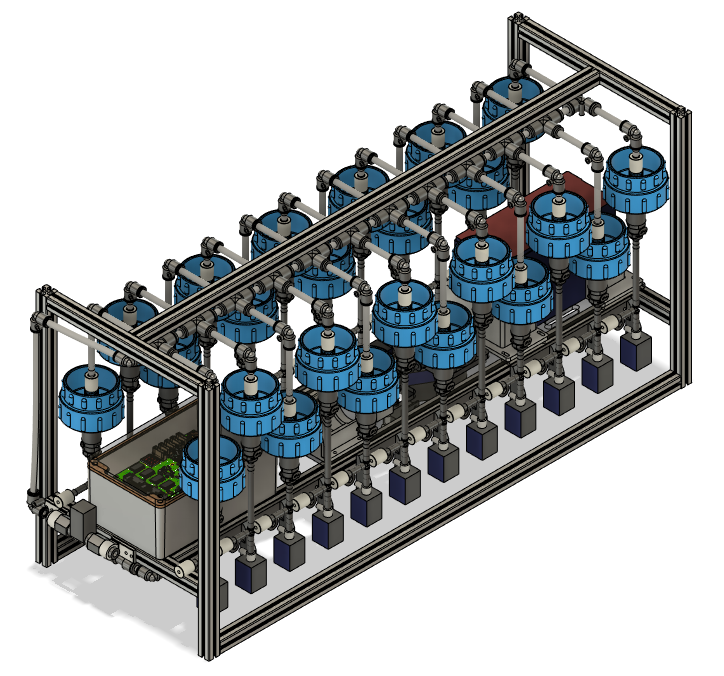
\includegraphics[scale=0.5]{./Assets/Sampler CAD.png} %Replace with actualy image?
\end{center}

\subsection{Hydraulics}
The hydraulics of the sampler can be roughly split into the following sections:
\begin{itemize}
	\item The Pump and Inputs
	\item The Lower Hydraulics
	\item The Filters
	\item The Upper Hydraulics and Outputs
\end{itemize}
There are three inputs into the sampler: one for air, one for preservative, and one for water. The preservative input is connected to a hydration bladder where the preservative of choice can be stored. The water input has a prefilter at the front end of the tube to prevent debris from entering the sampler. Three valves are used to control the flow from these inputs with the air preservative being regulated by a solenoid valve and the water being controlled by a ball valve. These three valves connect into a single tube connected to the input of the peristaltic pump.
The pump is capable of 400ml/min of flow under ideal conditions. The output of the pump connects directly into the Lower Hydraulic Rail. 

\begin{center}
	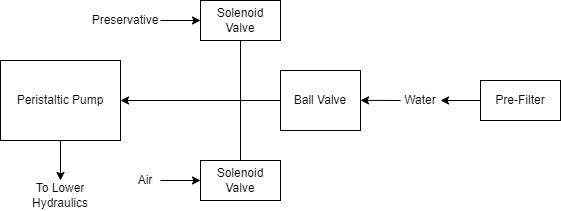
\includegraphics[scale=0.75]{./Assets/PolyWAG_HX_HD_InHydr.png}
\end{center}

The Lower Hydraulic Rail consists of 24 solenoid valves connected parallel to each other which controls which filter liquid flows through. The valves are split into two sets, one on each side of the sampler. In between these two sets is a M32JM-000105-100PG pressure and temperature sensors. The temperature is logged for later use and the pressure is used for monitoring, stopping an operation if the pressure exceeds a certain margin. At the end of the Lower Hydraulic Rail is another solenoid valve which allows for the lower hydraulics to be purged of their current contents when necessary.

\begin{center}
	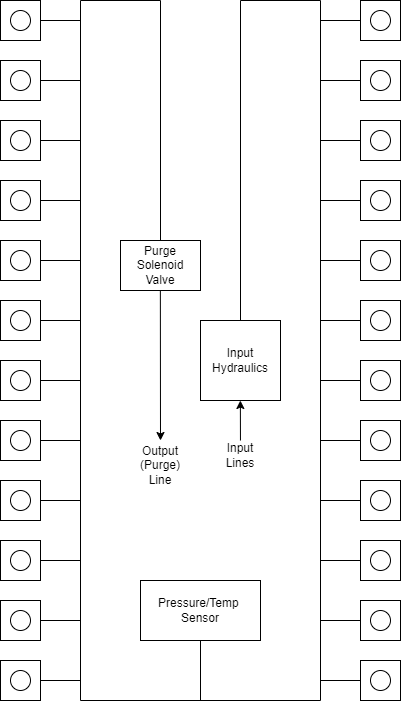
\includegraphics[scale=0.65, angle=-90]{./Assets/PolyWAG_HX_HD_LHR.png}
\end{center}

After the solenoid valve there is a tee connection that goes to a one-way check valve and a modified Advantec filter. The one-way check valve allows air into the solenoid valve that opens when the pump runs backwards. The Advantec filter is modified with a CPC quick disconnect and a one-way check valve. The one-way check valve is connected to the Upper Hydraulics and is used to prevent liquid from going backwards through the filter. The Upper Hydraulics simply connects the output of all the filters to one central line that goes through a flow meter and out of the sampler. 

\begin{center}
	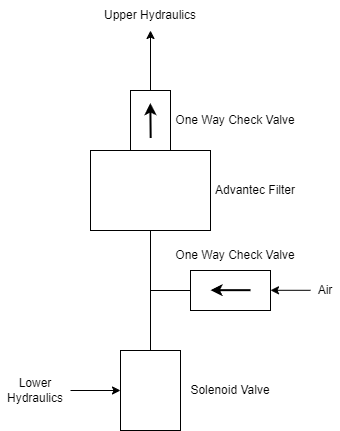
\includegraphics[scale=0.75]{./Assets/PolyWAG_HX_HD_Filter.png}
\end{center}

\subsection{Sampling Procedure}
Having worked on multiple iterations of the sampler, we have decided to go with a 13-step sampling sequence that helps reduce cross contamination significantly. This sequence can be split into 9 unique steps: Idle, Prefilter Clear, Flush, Offshoot Clean, De-pressure, Sample, Preservative Flush, Preservative, Air Flush, and End.

\begin{center}
	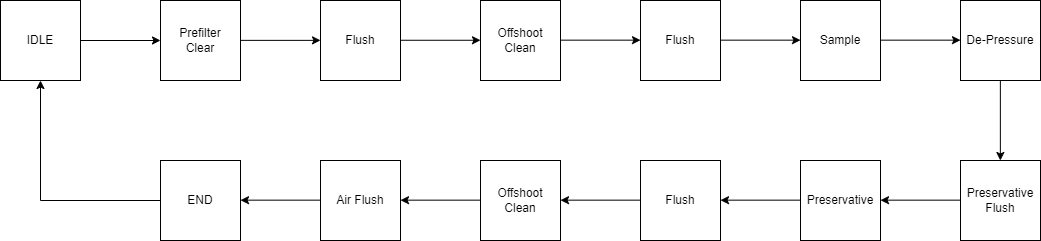
\includegraphics[scale=0.45]{./Assets/Sampling Sequence.drawio.png}
\end{center}

The Idle state is the default state of the sampler. This is where the sampler waits for a signal from the RTC to move to the first/next state of the Sampling Sequence. If the sampler is not in sleep mode, this is when a client would interact with the UI to do a handful of tasks such as setting up a Sampling Schedule or using the other task utilities. If the sampler is in sleep mode, then only the RTC and supporting circuits are powered. This means there is no way to interact with the sampler without exiting sleep mode.
\newline\par
Once the RTC sends the signal to start a sample procedure, the sampler enters the Prefilter Clear (PC) state. In this state, the purge and input ball valve are opened, and the pump is run in the backwards direction. This will allow for air to flow from the purge and out the input line. This is used to clear the prefilter of anything that might be clogging it, such as accumulated debris. This state runs for X seconds, before moving onto the next state. 
\newline\par
The Flush state and the proceeding Offshoot Clean (OC) state are used to prepare the lower hydraulics before the Sample state. The Flush state starts with the purge valve and the ball valving opening, then the motor starts to run in the forward direction. This fills the lower hydraulics with sample liquid and clears out/dilutes and liquid that remained from previous sample. The Flush state runs for the time specified when the Sampling Schedule is created. We recommend a Flush time of 6 minutes. 
\newline\par
The OC state closes the purge valve and opens the filter valve (for the filter which is about to be used. The pump runs backwards for a few seconds. This clears anything that might be in the tube between the valve and the filter (what we refer to as the offshoot). The Flush state is run one more time before moving to the Sample state.
\newline\par
Like the name suggests, the Sample state is where the system pushes the sample water through the filter. This is done by opening the Filter and Ball Valve and running the pump in the forward direction. The system moves to the next state when the target Sample Volume is reached. This volume is measured by a Flow Meter on the filter output line. Ideally, the state is terminated when the target volume is reached. There is an additional condition that will end the Sample state and that is the Sample Time. This time cutoff was added since the filter clogs and the flow rate decrease rapidly during the sample process. To prevent the sample state running for too long, the time limit was implemented. Both conditions are set during task scheduling. Since the pressure greatly increases due to the clogged filter, the de-pressure state is used to reduce the pressure in the lower hydraulics to ensure that the valves can operate consistently.
\newline\par
The Preservative Flush (PF) and Preservative (P) states are the next states in the sequence after the de-pressure state. The PF state is nearly identical to the Flush state except the Preservative input valve is used instead of the ball valve. The goal of this state is to saturate the lower hydraulics with preservative, preventing additional sample water that may have been stored in the lower hydraulics from going through the filter. If this water was allowed through the filter, then the Sample Volume would be inaccurate by the end of the sequence. The P state is like the Sample state except preservative is the input fluid instead of sample water. This state runs for a time specified by the user during scheduling.  
\newline\par
After the P state, another Flush and OC state runs to purge the leftover preservative in the lower hydraulics. After these two states, an Air Flush (AF) state is run which is identical to the Flush and PF states but uses the air valve as the input instead of the other two inputs. This ensures that any liquid that is in the lower hydraulics is purged. 
\newline\par
After the AF state occurs, the system sets an RTC alarm for the time of the next sample. The system then moves into Idle and if the system was in sleep mode, then the system will go into its low power state.

\subsection{Utilities}

\begin{center}
	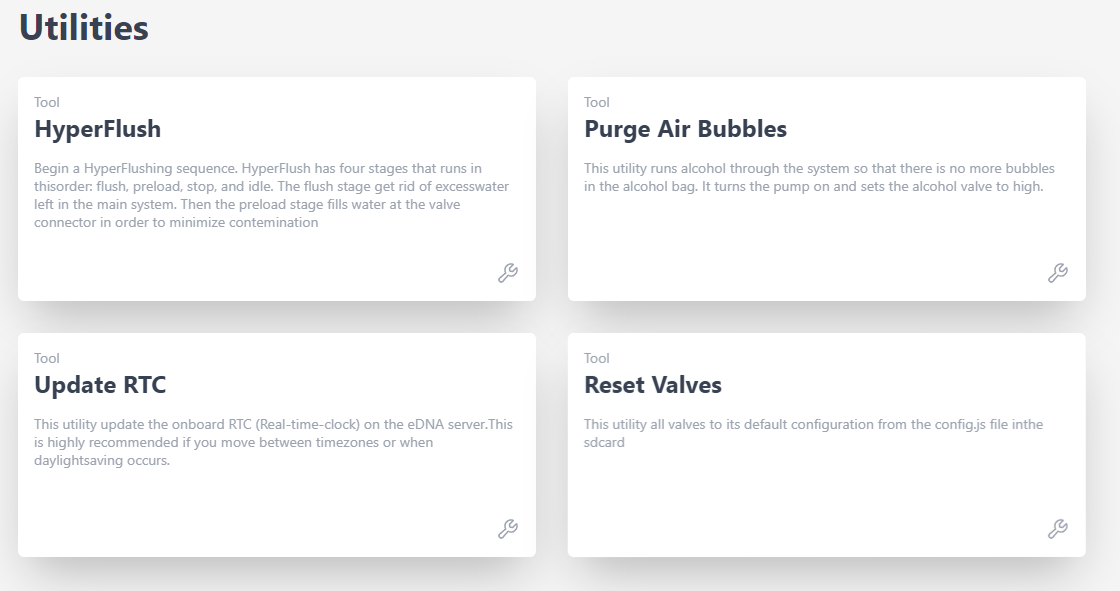
\includegraphics[scale=0.5]{./Assets/Utilities.png}
\end{center}

The HyperFlush utility runs water through every filter sequentially for a few seconds per filter. This is mainly used for cleaning out the system after a sample task (i.e., a set of 24 samples) to prevent any unwanted cross contamination. This utility can also be used to test the basic functionality of the sampler, as nearly every component is activated during this sequence. 
\newline\par
The Preservative Air Purge (PAP) utility turns the pump on and opens the alcohol valve for 10 seconds. This runs some alcohol through the system and removes air bubbles from the alcohol bag. Often it helps to use this utility multiple times and to tilt the Preservative Bladder so that the air is near the port.
\newline\par
The Update RTC utility is needed to make sure that the time on the sampler matches your local time, so scheduling a task will remain accurate. Whenever the system is fully depowered (ie the battery is removed), or when new code is uploaded to the microcontroller, the RTC will need to be updated. It is also recommended that the RTC is updated when there is a daylight-saving change, or when you move between time zones.
\newline\par
The Reset Valves Utility is used when valves have been sampled that you want to be sampled again. This is required since the system ‘locks’ the filter valves when they have been used in a sample, this prevents samples from being corrupted accidentally. The code does not let you sample a valve multiple times without being reset to prevent messing up a sample. It is important to note that this utility will reset all valves, not a specific one.

\subsection{Electronics}
\begin{center}
	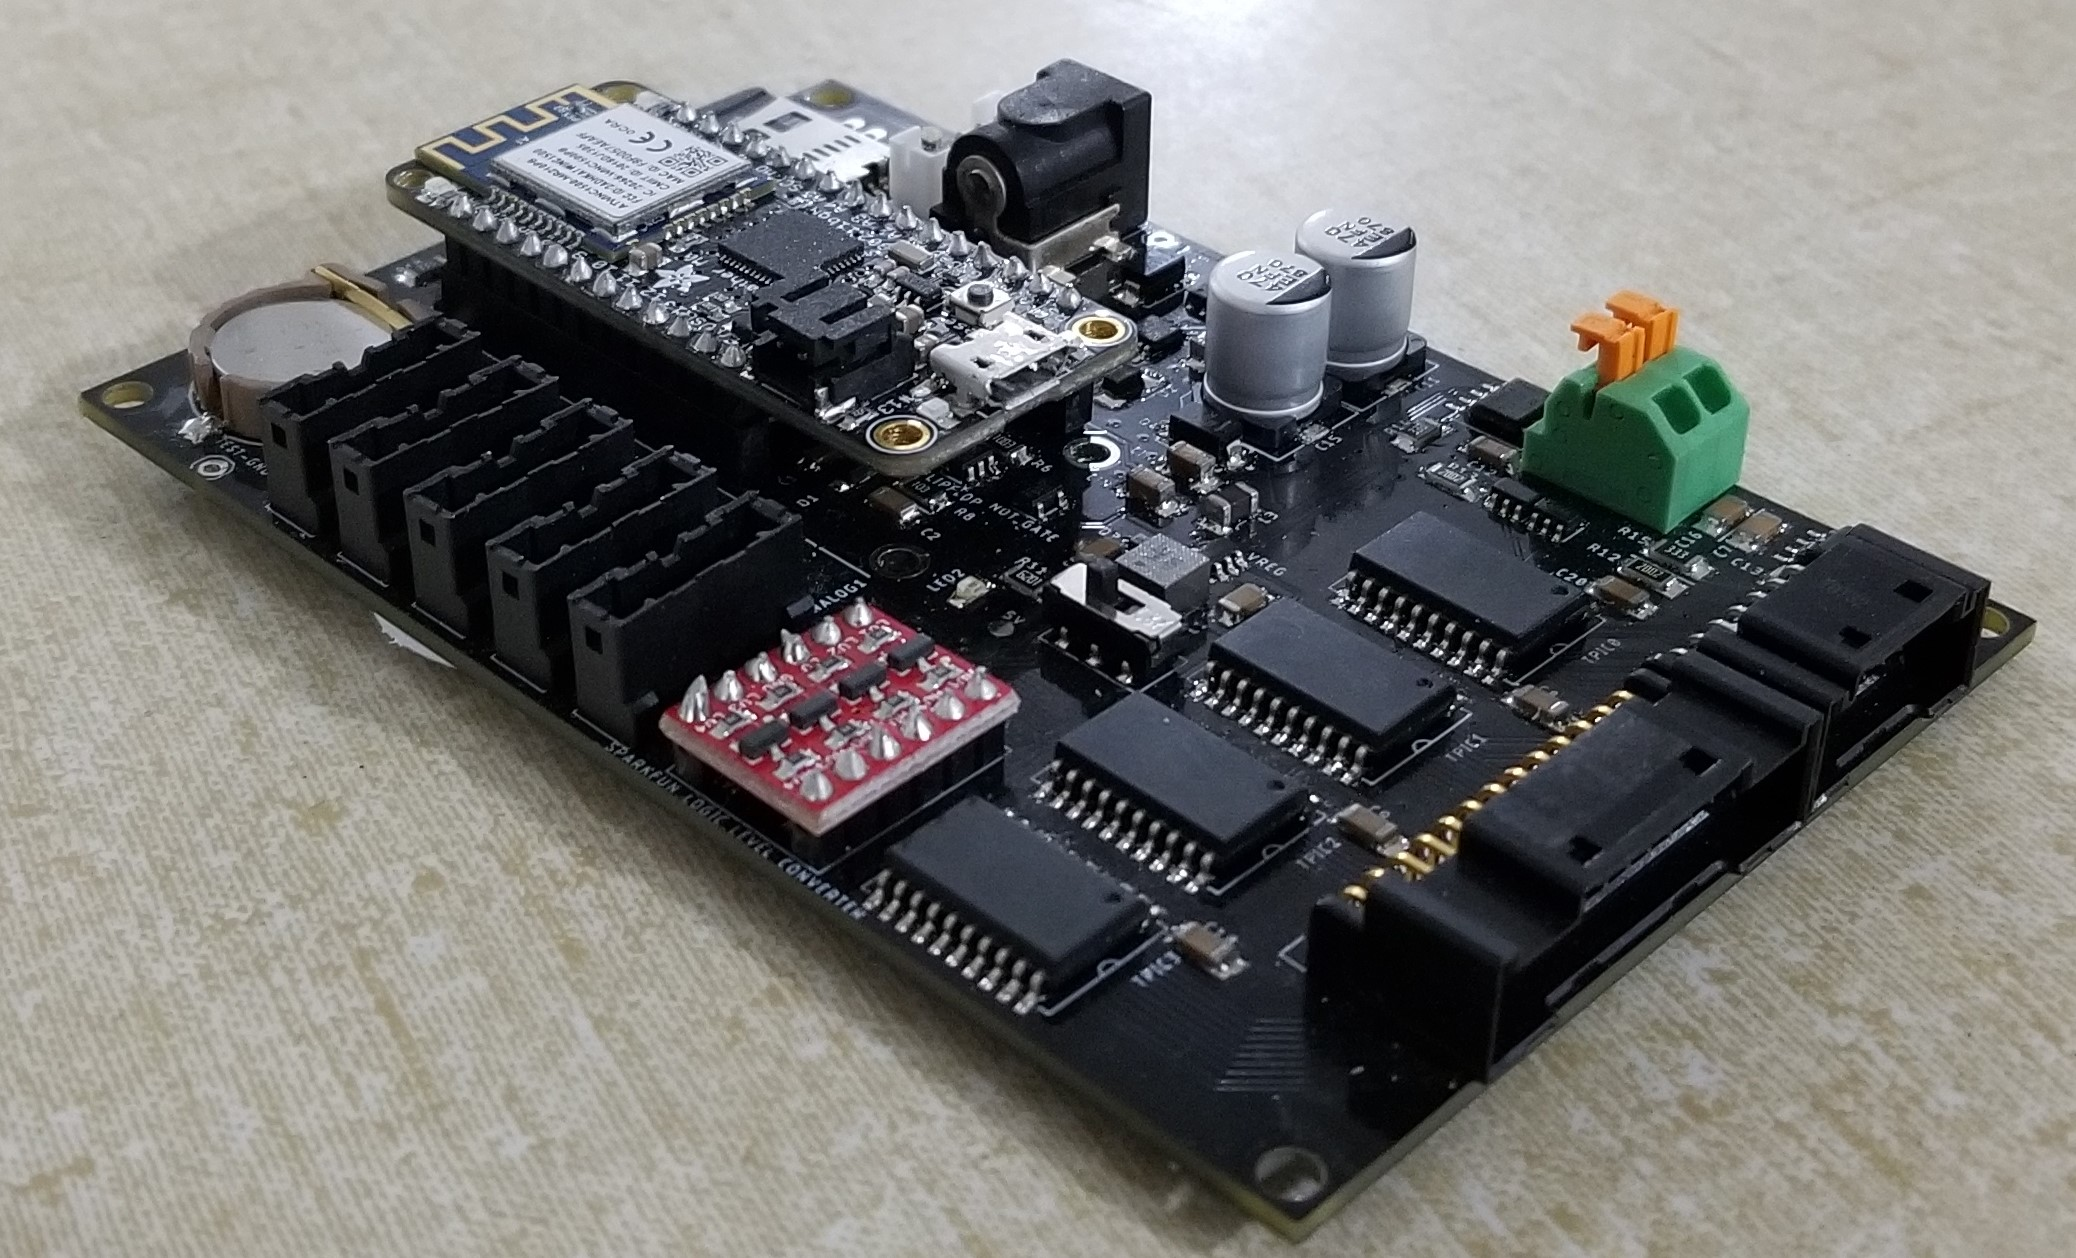
\includegraphics[scale=0.15]{./Assets/eDNABoard.jpg}
\end{center}

The PolyWAG Sampler is designed with a custom electronics control board that can be split into 8-10 blocks with an Adafruit Feather M0 at its core. These blocks consist of the microcontroller/Wifi Block, Power, RTC, and sleep control blocks, and the output blocks consisting of the Shift Register, Pump, and Ball-Valve H-Bridge Blocks. 

\begin{center}
	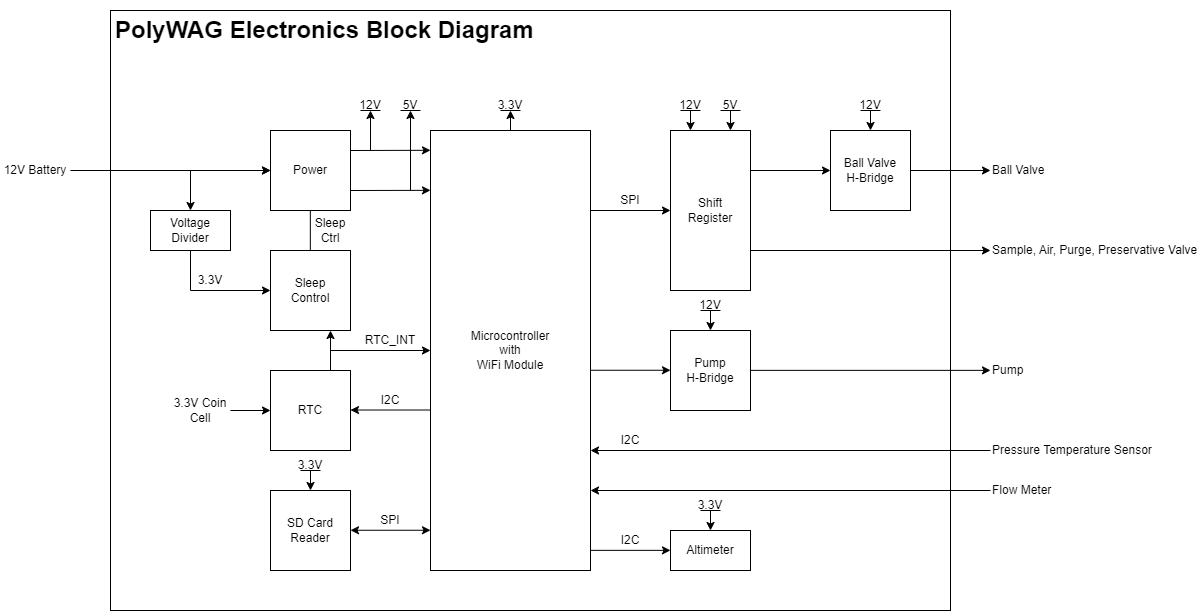
\includegraphics[scale=0.4]{./Assets/Electronics Block Diagram.png}
\end{center}

The power block consists of a reverse polarity current (RPC) circuit and a voltage regulator circuit. The RPC Circuit was added to protect the 12V battery from current flowing backwards through the system. While the battery has its own protection circuits, they lock the battery in the case of a short and need to be reset using the battery charger. The RPC circuit was added to prevent any “permanent” power loss while in the field. The voltage regulator circuit is a 12V to 5V regulator with an enable pin that connects to the sleep control circuit. This is used to save power during long term deployments. 
\newline\par
The RTC and sleep control circuit are used to keep track of time and to save power respectively. The sleep control circuit controls the output of the power circuit and is constantly being power by a simple voltage divider circuit. It is basically a Flip Flop circuit that is reset when the RTC triggers an interrupt. The RTC circuit is used to keep track of the time between samples and is powered by a coin cell while power is off. This allows it to keep accurate track of time and signals an interrupt when its internal alarm is triggered. This interrupt is used to both turn power back on and to inform the microcontroller that it is time for a sample. If noise causes the sleep control circuit to reactivate power, the microcontroller will see that the RTC did not trigger the interrupt and will fall back into power saving mode. 
\newline\par
The shift register circuit consists of 4 8-bit shift registers connect to the microcontroller via SPI. The shift registers are pull-down style shift registers where the ‘output’ pins are pulled to ground. This allows the shift registers to control devices that use higher logic voltages. This allows us to control the 27 12V solenoid valves with a 5V IC. The shift registers are also used to control the H-bridge for the Ball valve. The H-bridge for the pump is controlled directly by the microcontroller itself. 
\newline\par
The board contains an SD Card circuit for datalogging purposes. The data is logged every second and includes the current state, time, and data from the sensors. The sensors include an in-line pressure temperature sensors for monitoring the lower hydraulic line and a flow meter out the output for measuring volume.
\newline\par
The microcontroller of choice is an Adafruit Feather M0 WiFi. The WiFi version of the Feather M0 was chosen as the user interface requires the feather to host a webserver. 


\subsection{User Interface}

\begin{center}
	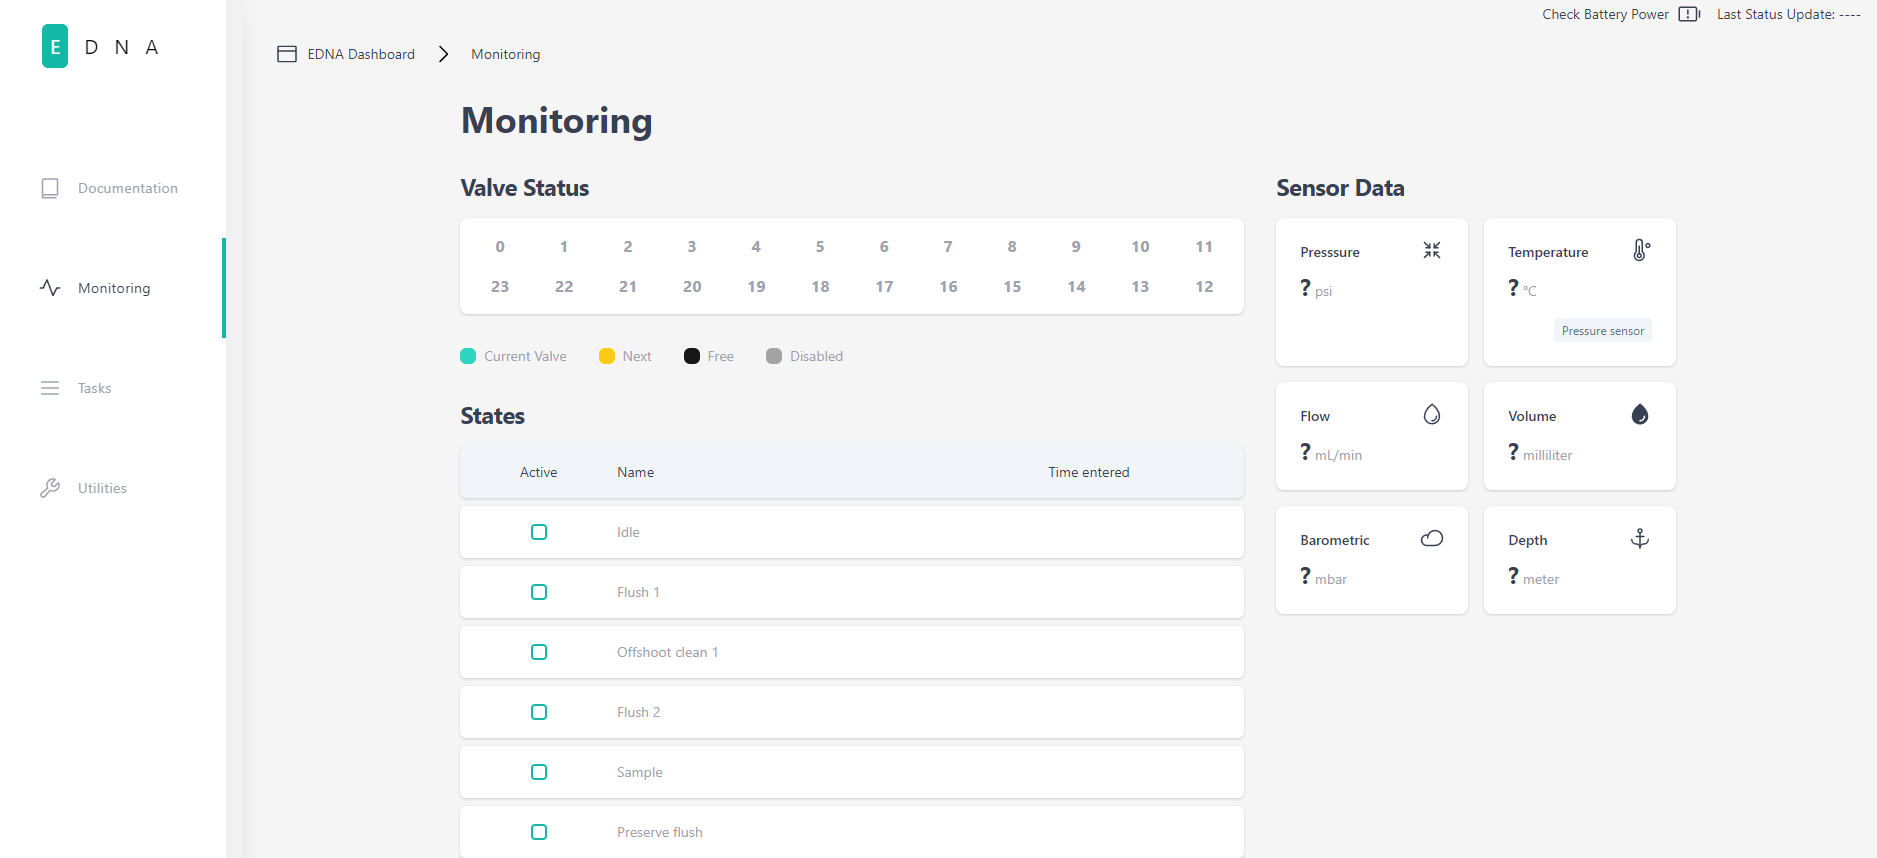
\includegraphics[scale=0.35]{./Assets/UI.png}
\end{center}

PolyWAG Sampler hosts a webserver that can be connected to via a browser. This acts as the user interface for the system. There are three main sections that make up the user interface: monitoring, tasks, and utilities. The monitoring page displays the data from the sensors, the current state of the sampling procedure, and information on the sampling valves such as the current valve being sampled, and which valves are locked and unlocked. The utilities page is used to activate the utilities mentioned earlier. The tasks page is where sampling tasks are created. Multiple tasks can be created, and each task is saved in memory for later modification and use. This page is also where tasks can be scheduled for sampling. Each task contains the information on which valves are being used as well as for how long each state occurs. 


\subsection{Task Configuration}

\section{Design Files Summary}
%
% Design Files
%
% > The  complete  design  files  must  be  either  uploaded  to  an  approved  online  repository,  uploaded  at the  time  of  submission  on  the  online  Editorial  Manager  submission  interface  as  supplementary materials [CAD files, videos,. . . ], or included in the body of the manuscript [e.g.  figures].  The three approved  online  repositories  are  Mendeley  Data,  the  Open  Science  Framework,  and  Zenodo. See repository instructions: https://doi.org/10.5281/zenodo.3346799

% > Design files should be in preferred format for making modifications. See OSHWA’s open-source definition for details: https://www.oshwa.org/definition/

% > Your design files should be editable - see {https://www.oshwa.org/definition/}{OSHWA’s open source definition of ‘Documentation’} for further details. You must then either:
% > > Upload your design files to one of the three approved online repositories - {https://data.mendeley.com/}{Mendeley Data} {https://doi.org/10.5281/zenodo.3346799}{instructions}), the {https://osf.io/}{Open Science Framework} ({https://osf.io/wgk7q/wiki/home/}{instructions}) or \href{https://zenodo.org/}{Zenodo} (\href{https://doi.org/10.5281/zenodo.3346799}{instructions}). We recommend this option as the repositories support versioning of files.
% > > Upload your design files as supplementary materials (e.g., CAD files, videos…) to Hardware X’s online editorial system when you submit your manuscript.
% > > Include your design files in the body of the manuscript (e.g., as figures).

%
% > The complete design files must be either uploaded to an approved online repository, uploaded at the time of submission on the online {https://editorialmanager.com/ohx/}{Editorial Manager} submission interface as supplementary materials [CAD files, videos,\dots], or included in the body of the manuscript [e.g. figures]. The three approved online repositories are {https://data.mendeley.com/}{Mendeley Data}, the {http://osf.io}{Open Science Framework}, and {https://zenodo.org/}{Zenodo}. See repository instructions {https://doi.org/10.5281/zenodo.3346799}{here}. Design files should be in preferred format for making modifications. See {https://www.oshwa.org/definition/}{OSHWA’s open-source definition} for details.

% > CAD files: You are encouraged to use free and open source software packages for creating the files. For CAD files, {http://www.openscad.org/}{OpenSCAD}, {http://www.freecadweb.org/}{FreeCAD}, or {https://www.blender.org/}{Blender} are encouraged, but, if these are not available, we accept source files from proprietary CAD packages, such as Autocad or Solidworks, and other drawing packages.

% > {3D printing: Supplementary files that facilitate digital replication of the devices are encouraged;  for example, STL files for 3D printing components. We recommend uploading CAD files to the {http://3dprint.nih.gov/}{NIH 3D Print Exchange} as Custom Labware and then entering the link here.}

% > Electronics: PCB layouts and other electronics design files can be uploaded to the {http://www.ohwr.org/}{Open Hardware Repository} or other repositories or as supplementary materials.}

% > Software and firmware: All software files used in the design and operation of the hardware should be included in the repository. Provide a description of the software and firmware and use extensive comments in the code.


%
% Design Files Summary
%
% > Complete a separate row for each design file associated with your hardware (including the primary design files). Any empty rows should be deleted.}
% Please include a summary of all design files for your hardware by filling rows of the table below
% > For example: 
%	Design file 1 & 
%	e.g. CAD file, figures, videos & 
% 	All designs must be submitted under an open hardware license. Enter the corresponding open source license for the file. & 
%	Either enter the URL for the repository or the sentence: "Available with the article".


\vskip 0.1cm
\tabulinesep=1ex
\begin{tabu} to \linewidth {|X[l]|X[l]|X[1.5,1,l]|X[1.5,1,l]|} 
	\hline
	\textbf{Design filename} & \textbf{File type} & \textbf{Open source license} & \textbf{Location of the file} \\\hline
	% Design file & File type & License & Link \\\hline	
	
	% General CAD
	CAD Assembly 				& CAD file & \dots & \dots \\\hline
	% 3D Printed
	Battery Bracket 			& CAD file & \dots & \dots \\\hline
	Sample Valve Mount 			& CAD file & \dots & \dots \\\hline
	Preservative Valve Mount 	& CAD file & \dots & \dots \\\hline
	Flow Meter Mount 			& CAD file & \dots & \dots \\\hline
	Tube Guide 					& CAD file & \dots & \dots \\\hline
	% Acrylic
	Central Assembly Mount		& CAD file & \dots & \dots \\\hline
	Control Board Mount 		& CAD file & \dots & \dots \\\hline
	Electronics Box Lid			& CAD file & \dots & \dots \\\hline %???
	% EDA
	Control Board Schematic		& EDA file & \dots & \dots \\\hline
	Control Board PCB			& EDA file & \dots & \dots \\\hline
	Switch Breakout Schematic	& EDA file & \dots & \dots \\\hline
	Switch Breakout PCB			& EDA file & \dots & \dots \\\hline
	% Software
	UI Code 					& Software & \dots & \dots \\\hline
	Device (Server) Code 		& Software & \dots & \dots \\\hline
\end{tabu}


% For each design file listed in the summary above, include a short description of the file below (one or two sentences)
\vskip 0.3cm
\noindent
\begin{itemize}
\item 
The CAD Assembly is a CAD file with every major components. The tubing and minor things such as zip ties for cable routing are not included. 
\item 
The Battery Bracket is a 3D-Printed component to hold down the battery during transit. Paired with a Velcro strap, the battery does not move.
\item 
The Sample Valve Mount is a 3D-printed bracket that holds four solenoid valves. There are six brackets in the sampler and each valve corresponds with a filter. 
\item 
The Preservative Valve Mount is a 3D-printed component that holds the preservative valve in place. 
\item 
The Flow Meter Mount is a 3D-printed bracket that holds the flow sensor to the frame.
\item 
The Tube Guide is a 3D-printed components that helps hold the input and output tubes in place. 
\item 
The Central Assembly Mount is a laser-cut acrylic components that all of the "central" components mount to. This includes the pump, input control valves, and the battery. 
\item 
The Central Board mount is a laser-cut acrylic components that the allows the main control board to mount inside the electronics box.
\item 
The electronics box lid is a CNCed Acrylic components that replaces the metal lid but maintains the groove for the gasket.
\item 
The Control Board Schematic and PCB are EDA files in the Autodesk EAGLE format for the sampler's main control board. 
\item 
The Switch Breakout Schematic and PCB are EDA files in the Autodesk EAGLE format for the sampler's main power switch. 
\item 
The UI Code consists of all the raw files needed to compile the UI that is seen when operating the sampler. The compiled version of the UI is stored in the sampler's SD Card.
\item 
The device (server) code is the code that is uplaoded to the microcontroller and handles all of the sampler's functions. The code is split into multiple different files each handling a specific task. 
\end{itemize}

\section{Bill of materials}
% For a complex Bill of Materials, the complete Bill of Materials (editable spreadsheet file e.g., ODS file type or PDF file) can be uploaded in an open access online location such as the Open Science Framework repository. Include the link here. Alternatively, the Bill of Materials can be uploaded at the time of submission on the online Elsevier submission interface as supplementary material.

% > To make it easy to tell which item in the Bill of Materials corresponds to which component in your design file(s), use matching designators in both places, or otherwise explain the correspondence.

% > For material type, select from: Metal, semi-conductor, ceramic, polymer, biomaterial, organic, inorganic, composite, nanomaterial, semiconductor, non-specific, or other 

% > \href{https://osf.io/}{\underline{Open Science Framework}} 
Given the number of materials required to build a PolyWAG Sampler, The BOM will be located in an external file and can be found \href{https://docs.google.com/spreadsheets/d/1WZbGYL1k3ne1a8Z1YOA0necr3MgxMj_BiEK7JuaGnzE/edit#gid=1118434588}{\underline{here}}
% Change the link for one that points to Zenodo
% > Add the BOM to Zenodo


\section{Build instructions}
%Provide detailed, step by step instructions for the construction of the reported hardware include all necessary information for reproducing the submitted hardware.
% > Explain and, when possible, characterize design decisions. Including design alternatives if they exist. 
% > Use visual instructions such as schematics, images, and videos. 
% > Clearly reference design files and component parts described in the Design File Summary and Bill of Materials. 
% > Highlight potential safety concerns that may arise

Given the complexity of the PolyWAG Sampler, a Build Instructions section of sufficient detail would be near a hundred pages long. This is why an external build guide document will be linked for those who are interested in knowing how one of these samplers are assembled. This file can be located \href{https://drive.google.com/file/d/1QSpYj-N6-jE-VbXLVelzRzzdIF1lMkuC/view?usp=sharing}{\underline{here}}
% Change the link for one that points to Zenodo
% > Add the Build Guide to Zenodo

\section{Operation instructions}
% Provide detailed instructions for the safe and proper operation of the hardware. 
% > Step-by-step operational instructions for operating the hardware. 
% > Use visual instructions as necessary. 
% > Highlight potential safety hazards.

%%% Kai's Notes: %%%
%%% Use Mark's section here
%%% Maybe add a section for physically using the sampler. 


\section{Validation and characterization}
%Demonstrate the operation of the hardware and characterize its performance over relevant critical metrics
%> Demonstrate the use of the hardware for a relevant use case. 
%> If possible, characterize performance of the hardware over operational parameters. 
%> Create a bulleted list that describes the capabilities (and limitations) of the hardware. For example consider descriptions of load, operation time, spin speed, coefficient of variation, accuracy, precision and etc. 

%%% Kai's Notes
%%% Insert Riley's Section once edits are made. 

The PolyWAG Sampler was tested by the Openly Published Environmental Sensing Lab at Oregon State University. It was characterized by a blend of isolated in-lab testing procedures as well as field tests on the Willamette River and the Irish Bend Covered Bridge In Corvallis, Oregon. To assess the capabilities of the sampler, the following evaluations were conducted: to establish the viability of field deployment at running water sources in Alaska.

\subsection{Cross-Contamination Testing}

The primary use case of the PolyWAG eDNA sampler is for use in water sampling to capture existing trace biological information in the form of DNA by means of filtration. In gauging the use case of the sampler for eDNA collection and characterization, we subjected the sampler to a lengthy cross-contamination study for detecting residual DNA in subsequent sample steps. Prior to sampling, a cleaning and sterilization process was conducted to eliminate any sources of contamination from previous testing. After running the sampling procedure, the results were evaluated by means of Polymerase-chain reaction (PCR).
\newline\par
The basis for these observations is the use of Alaskan Sockeye Salmon DNA. To obtain Alaskan Sockeye Salmon DNA, 1 filet of salmon (~500g) is placed in an 8 gallon container of DI Water and left for 24 hours. During this time, biological material diffuses into the bulk water. After 24 hours the remaining salmon mass is removed to ensure constant salmon DNA concentration across trials.
\newline\par
The sample cleaning procedure makes use of the sampler’s HyperFlush utility to sterilize both the filter housings and the sampler hydraulic lines. The HyperHlush utility flushes each valve of the system sequentially with any bulk liquid connected to the input line. The cleaning procedure makes use of three HyperFlush cycles in the following liquid order: DI water, 6\% bleach, 5\% ascorbic acid. These cycles are repeated three times and followed by three subsequent HyperFlush cycles of DI water to purge all residual chemicals
\newline\par
The sampling procedure for cross-contamination characterization makes use of a sample of DNA followed by subsequent samples of DI Water. To establish experimental controls, the first sample of the study is a negative control containing DI water. This negative control gauges the success of the cleaning protocol, ensuring no prior contamination. Following this control, the process consists of three subsequent samples: Fish water (Positive Control) and two samples of DI water. Separate inlet lines are used for DI water and fish water to isolate the source of cross-contamination to the sampler itself, the lines being switched manually between samples. The data collected during this study consists of four trials performed using the following task settings on the eDNA UI: 1000 mL max sample volume, 4-minute max sample time, 10-second preservative flush, and 12-minute flush time (~5L). After sampling, the samples were individually packaged and sent for PCR analysis. 
\newline\par
For PCR analysis, the cellulose nitrate filters containing the salmon DNA are dissolved releasing the trapped DNA into solution. Sockeye Salmon primers were added to the DNA solution. During PCR the DNA is amplified on a scale of 109 times the original DNA concentration.  From here, immuno-fluorescence is used to quantify the amount of DNA retrieved by measuring the intensity of light emitted by the sockeye-salmon DNA. These values are interpreted in terms of a CT score. CT scores between 0-40 CT indicates the presence of Salmon DNA, while a CT score >40 indicates no Salmon DNA is detected.
\newline\par
Using these processes 13 samples were taken using the sampler. This included 1 Negative control, and 4 sample trials.

\vskip 0.2cm
\begin{center}
\tabulinesep=1ex
\begin{tabu} to \linewidth {|X|X|X[2,l]|}
	\hline  
	\textbf{Sample Name} & \textbf{CT} & \textbf{Results}
  	\\
  	\Xhline{4\arrayrulewidth} 
  	Negative Control & 39.65583038 & \textbf{Positive-Low Quantity(1/2, high Ct)}
  	\\
  	\hline 
  	Negative Control & Undetermined &
  	\\ 
	\hline 
  	Positive Control & 29.15957832 &
  	\\ 
  	\hline 
  	Positive Control & 29.47208214 & \textbf{Positive}
  	\\ 
	\hline 
  	Trial 1: Sample 1 & Undetermined & \textbf{}
  	\\ 
	\hline 
  	Trial 1: Sample 1 & Undetermined & \textbf{Negative}
  	\\ \hline 
  	Trial 1: Sample 2 & Undetermined & \textbf{}
  	\\ \hline 
  	Trial 1: Sample 2 & Undetermined & \textbf{Negative}
  	\\ 
  	\Xhline{4\arrayrulewidth} 
  	Positive Control & 30.94010544 & \textbf{Positive}
  	\\ 
  	\hline 
  	Positive Control & 30.6325016 & \textbf{Positive}
  	\\ 
	\hline 
  	Trial 2: Sample 1 & Undetermined & \textbf{}
  	\\ 
	\hline 
  	Trial 2: Sample 1 & 39.86541748 & \textbf{Positive-Low Quantity(1/2, high Ct)}
  	\\ 
  	\hline 
  	Trial 2: Sample 2 & Undetermined & \textbf{Negative}
  	\\ 
  	\hline 
  	Trial 2: Sample 2 & Undetermined & \textbf{Negative}
  	\\ 
  	\Xhline{4\arrayrulewidth}
  	Positive Control & 29.15957832 &
  	\\ 
  	\hline 
  	Positive Control & 29.47208214 & \textbf{Positive}
  	\\ 
	\hline 
  	Trial 3: Sample 1 & Undetermined & \textbf{}
  	\\ 
	\hline 
  	Trial 3: Sample 1 & 39.46964645 & \textbf{Positive-Low Quantity(1/2, high Ct)}
  	\\ 
  	\hline 
  	Trial 3: Sample 2 & Undetermined & \textbf{}
  	\\ 
  	\hline 
  	Trial 3: Sample 2 & Undetermined & \textbf{Negative}
  	\\ 
  	\Xhline{4\arrayrulewidth}
  	Positive Control & 29.15957832 &
  	\\ 
  	\hline 
  	Positive Control & 29.47208214 & \textbf{Positive}
  	\\ 
	\hline 
  	Trial 4: Sample 1 & Undetermined & \textbf{}
  	\\ 
	\hline 
  	Trial 4: Sample 1 & Undetermined & \textbf{Negative}
  	\\ 
  	\hline 
  	Trial 4: Sample 2 & Undetermined & \textbf{}
  	\\ 
  	\hline 
  	Trial 4: Sample 2 & Undetermined & \textbf{Negative}
  	\\ 
	\hline
\end{tabu}
\end{center}

The 4 trials conducted came to varying degrees of success. In trials one and four, the CT scores of the samples following the positive controls were undetectable. This indicates that there is no detectable DNA in the PCR-amplified sample. Samples two and three contained CT scores <40; however, in very low detectable quantities. In both cases, the sample immediately following the control are the samples in question. In the duplicate amplification one trial contained a CT score between 39 and 40 while the other was undetectable. This indicates a very faint presence of fish DNA between samples. The cause of this can be explained by two reasons. One is that the sampler is unable to prevent cross-contamination between trials. The other is that the cleaning cycle is not adequate for ridding all DNA in the sampler. The latter of the two seems more likely because of the negative control. Like the two barely detectable samples the negative control indicated a faint positive signal. This means one of two things: contaminated sample water or insufficient cleaning cycle. Based on these results the sampler does not justify evidence that the sampler prevents cross-contamination between samples. That being said there is evidence that the flushes between samples do minimize contamination. This is supported because sample two in all trials were identified as negative. Therefore, increasing the flush and cleaning times shows promise for mitigating cross-contamination issues.

\subsubsection{Turbidity}
To ensure the effective use of the sampler in non-ideal conditions, the sampler was analyzed by means of a flow analysis across a range of turbidity levels. The purpose of this test is to ensure adequate flow through the filter before it clogs. For eDNA purposes a minimum of 500 mL of filtered volume is required to accurately analyze the DNA concentration of the input stream. For testing, a 5.0 um filter and 75 um pre-filter are evaluated.
\newline\par
Based on water turbidity data for Alaskan streams in April, the turbidity of the water ranges from ~30-80 NTU. To reproduce this range, a 2000 NTU formazin based turbidity standard was diluted to produce 3L of the following NTU standards: 50, 100, 250 NTU. These turbidity standards were mixed within a beaker with a 2-inch stir bar at the lowest speed that a vortex was observed. The 75 um system pre-filter was suspended two inches from the bottom of the beaker while sampling. Sampling was conducted and stopped once the flow rate dropped below 60 mL/min. This drop in flow rate indicates a filter clogging.

\begin{center}
	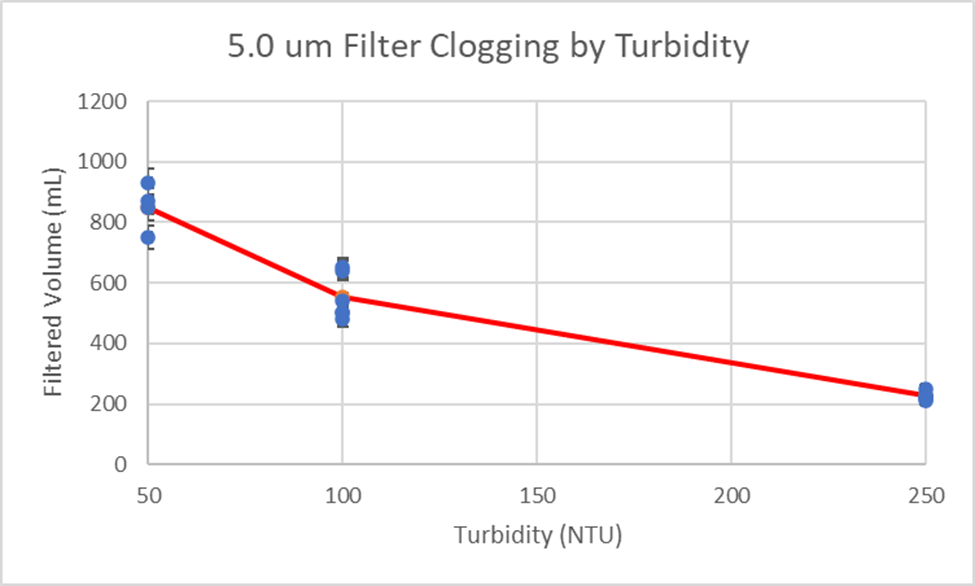
\includegraphics[scale=1]{./Assets/Turbidity.png}
\end{center}

To gauge the effectiveness of the sampler in the different turbidites the values are compared to the 500 mL minimum filtered volume. Greater than 500 mL of filtered volume indicates a successful sampler run at that water quality. As a result of this testing, the sampler is found to successfully operate in the range of 30-80 NTU. The data indicates the sampler can run in water qualities up to 100 NTU before samples under 500 mL are observed. Subsequent testing at 250 NTU indicates for lower-quality water streams, the sampler’s function decreases substantially, only filtering 200-250 mL per filter.This indicates that the sampler’s peristaltic pump is not able to build a high enough pressure gradient across the filter. Therefore for environments with lower water quality an increase in pump power is needed.
\newline\par
After conducting idealized laboratory trials, the sampler was placed in the field to test the flow for real-world applications. The sampler was placed in two locations in Corvallis, Oregon: the Irish Bend Covered Bridge on Oak Creek, and the Willamette Boat Landing on the Willamette River. In both locations, the sampler was deployed on the shore of the river with an inlet hose that ran to faster-moving water. For Oak Creek, the sampler’s prefilter was staked 4 inches between the water level in the middle of the stream. For the Willamette River, the inlet hose was immobilized at the end of the Willamette landing boat launch dock. The purpose of this trial is to serve as a proof of concept of the device in real world water streams. In both Oak Creek and the Willamette River, three trials were conducted in series to investigate the effects of non-idealized real world conditions on the sampler. The success of these trials is based on the ability to achieve greater than 500 mL of filtered volume per sample. The two rivers provide variable conditions on the quality of the water. Oak Creek contains low river flow and high water quality, while the Willamette river was experiencing flooding with very murky, low water quality. Without a turbidity sensor, the relative turbidity of these streams were determined relative to the observed turbidity standards used for the lab turbidity testing.

\vskip 0.2cm
\begin{center}
\tabulinesep=1ex
\begin{tabu} to \linewidth {|X|X|X|X|}
	\hline  
	\multicolumn{4}{|c|}{Filtered Volume Field Testing}
  	\\
  	\hline 
  	Trial & Location & Volume (mL) & Turbidity (NTU)
  	\\ 
	\hline 
  	1 & Oak Creek & 523 & $<$100
  	\\ 
	\hline 
  	2 & Oak Creek & 750 & $<$100
  	\\ 
	\hline 
  	3 & Oak Creek & 810 & $<$100
  	\\ 
	\hline 
  	4 & Willamette River & 270 & $>$1000
  	\\ 
	\hline 
  	5 & Willamette River & 300 & $>$1000
  	\\ 
	\hline 
  	6 & Willamette River & 340 & $>$1000
  	\\ 
	\hline
\end{tabu}
\end{center}

As a result of these trials, the sampler performed in much the same way as the lab turbidity trials. For the lower turbidity water sources the sampler had no issues reaching over 500mL of filtered volume. For the higher turbidity sources the 500 mL filtered volume minimum was not met; however, this was expected of the trial. Altogether, these results confirm the use case of the sampler in low turbidity environments.

\subsubsection{Flow Accuracy Testing}

The kinematic viscosity of water varies with temperature. This indicates that the sampler will read different values for flow rate for different temperatures. To ensure the sampler the flowmeter provides accurate flow readings for the upcoming Alaskan trials, the sampler was calibrated to reach accurate flow readings between 3-5’C. For accurate eDNA measurements the accuracy of the filtered volume must be within 10\% of the true filtered volume. Using the 10\% value as an end condition, several trials were conducted to determine the optimal volume constant for the flow meter pulses. In these trials, the outlet of the sampler is manually measured with a graduated cylinder and compared to the sampler’s calculated value.The percent error was then calculated between the two quantities. To ensure accuracy across the sampler’s operating range, the filtered volume was measured and compared at 250, 500, and 1000 mL for each volume constant. By averaging these values at each volume constant the average error per volume constant was discovered. 

\begin{center}
	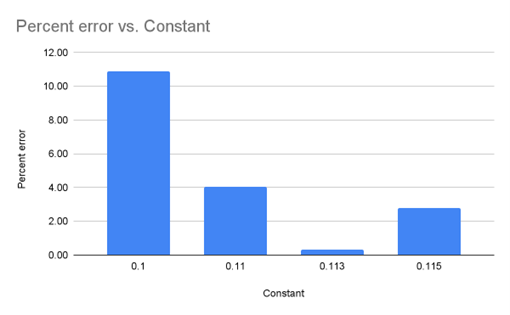
\includegraphics[scale=1]{./Assets/Flow1.png}
\end{center}

The results determined from this process indicate the constant that is centered within the error. In other words, the smaller the bar the more the positive and negative errors negate each other. This essentially centers the solution in the error domain. The minimum error indicates an ideal volume constant at or near 0.113. This alone does not demonstrate the accuracy of the volume measurement. Rather this indicates the most normalized variability between the trials. When looking at the max error between trials the hard limit of 10\% places these values in context.

\begin{center}
	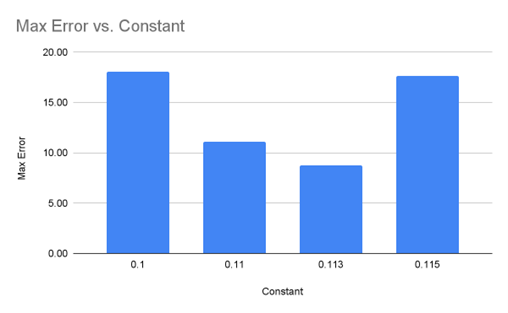
\includegraphics[scale=1]{./Assets/Flow2.png}
\end{center}

When viewing the max magnitude of error, a convex solution with a minimum error between real and observed volumes. In this context, the minimum absolute error is also easily determined to be at volume constant 0.113. The max error at this measurement falls below the 10\% threshold, indicating the sampler’s viability for eDNA collection purposes.

\subsubsection{Battery Life Testing}
Battery life varies with the ambient temperature of the surrounding environment \cite{art:Battery}. To gauge the battery life of the sampler in a cold Alaskan environment the battery was placed in a freezer at 0’C. The battery was left for two weeks to simulate the two-week field deployment time in Alaska. After two weeks, the battery line was plugged into the sampler while remaining in the freezer. A full 24-sample procedure was conducted. To ensure normal operating conditions the full 24-sample procedure was used using the default sampling procedure. Because the battery did not die during this time the sampler was determined to have enough battery life for normal operation of the sampler.


\section{Conclusion}
% Insert Short Conclusion Paragraph
% Reiterate Benefits
% Mention 

The PolyWAG Sampler shows a lot of promise when it comes to eDNA Sampling applications. This combined with the low cost of \$3800 for the materials makes the PolyWAG a potentially alternative to existing eDNA Samplers. Though the cross-contamination tests need to be redone to fully verify the sampler, even the existing results show a lot of promise. 
\newline\par
There are other improvements that can be made to the PolyWAG system outside of redoing some of the validation tests. This include new or improved features such as an increased the max sample volume and turbidity capability, Automatic Calibration for Water Viscosity based on Temperatur, as well as upgrading certain components to raise the specifications of the sampler, such as the flow meter, solenoid valves, and battery. 


\par\noindent\newline
\textbf{Ethics statements}\\
\noindent
The work does not use any human or animal subjects.\\


\noindent
\textbf{CRediT author statement}\\
% CRediT is in initiative that enables authors to share an accurate and detailed description of their diverse contributions to a published work.
% Example:
% Zhang San: Conceptualization, Methodology, Software. Priya Singh: Data curation, Writing- Original draft preparation. Wang Wu: Visualization, Investigation. Jan Jansen: Supervision. Ajay Kumar: Software, Validation. Sun Qi: Writing- Reviewing and Editing.
% Please add a CRediT author statement for your data article here, using the \href{https://www.elsevier.com/authors/journal-authors/policies-and-ethics/credit-author-statement}{categories listed on this webpage}.

\noindent
\textbf{Kai Roy}: Project administration, Hardware(Electrical), Validation, Writing- Original draft \\
\noindent
\textbf{Riley Prince}: Project administration, Methodology, Validation, Data curation, Writing- Original draft \\
\noindent
\textbf{Marc Belinga}: Software, Investigation, Writing- Original draft \\
\noindent
\textbf{Torrey Menne}: Conceptualization, Hardware\\
\noindent
\textbf{Bao Nguyen}: Project administration, Conceptualization, Hardware(Electrical)\\
\noindent
\textbf{Nikhil Wandhekar}: Project administration, Hardware\\
\noindent
\textbf{Nathan Jesudason}: Software, Validation \\
\noindent
\textbf{Kawin Pechetratanapanit}: Conceptualization, Software \\
\noindent
\textbf{John Selker}: Funding acquisition, Supervision \\
\noindent
\textbf{Chet Udell}: Funding acquisition, Supervision \\
\noindent
\textbf{Cara Walter}: Funding acquisition, Supervision, Resources \\

\noindent
\textbf{Auther}: Contribution. \\

\noindent
\textbf{Acknowledgements}\\
% [List here those individuals who provided help during the research (e.g., providing language help, writing assistance or proof reading the article, etc.).] Please also identify who provided financial support for the conduct of the research and/or preparation of the article and to briefly describe the role of the sponsor(s), if any, in study design; in the collection, analysis and interpretation of data; in the writing of the report; and in the decision to submit the article for publication. If the funding source(s) had no such involvement then this should be stated.}


\noindent
\textit{All contributors who do not meet the criteria for authorship should be listed in an acknowledgments section.} 
\vskip 0.2cm
\noindent
\textit{In addition, please list any funding sources in this section. List funding sources in this standard way to facilitate compliance to funder's requirements:}
\vskip 0.2cm
\noindent
\textit{Funding: This work was supported by the National Institutes of Health [grant numbers xxxx, yyyy]; the Bill \& Melinda Gates Foundation, Seattle, WA [grant number zzzz]; and the United States Institutes of Peace [grant number aaaa].}
\vskip 0.2cm
\noindent
\textit{It is not necessary to include detailed descriptions on the program or type of grants and awards. When funding is from a block grant or other resources available to a university, college, or other research institution, submit the name of the institute or organization that provided the funding.}
\vskip 0.2cm
\noindent
\textit{If no funding has been provided for the research, please include the following sentence:}
\vskip 0.2cm
\noindent
\textit{This research did not receive any specific grant from funding agencies in the public, commercial, or not-for-profit sectors.
}\\


%
% References
%
%> Include at least one reference, to the original publication of the hardware you customized.
%> Include other references as required. Include references to put your device in context in the literature. For more information on the reference format in HardwareX please see the Guide for Authors at: https://www.elsevier.com/journals/hardwarex/2468-0672/guide-for-authors
\bibliography{refs}
\bibliographystyle{IEEEtran}

\end{document}

%> Author manuscript checklist
%> ●	HardwareX is a journal dedicated to the exhaustive and fully open source communication of advances in scientific infrastructure. Upon submission the author declares that all information necessary to reproduce the subject of the submission (e.g. bill of materials, build instructions, calibration procedures, source files, code, and safety considerations) is communicated in full and is accessible for use under an open source license. 
%> ●	Is the subject of the submission under an open source license? Are design files in the preferred format for making modifications? As defined by the Open Source Hardware definition. 
%> ●	Can the hardware be reproduced with the details provided in the submission?
%> ●	Are all relevant design files available on Mendeley Data, the Open Science Framework, or Zenodo repositories, described in the Summary of Design Files document, and clearly documented? (e.g. descriptive file names, commented code, labeled images, etc.) 
%>      ○	If in the Open Science Framework, the repository has be registered? Instructions
%>      ○	If in Zenodo, the repository is open access and is published? Instructions
%>      ○	If in Mendeley Data, the repository is published or the sharable link was included in the additional information of the Editorial Submission interface? Instructions
%> ●	Are visual instructions used when necessary?
%> ●	Is the utility of the hardware to the scientific community? Has a specific scientific application been demonstrated using the hardware?
%> ●	Is the performance of the hardware adequately demonstrated and characterized?
%> ●	Are all potential safety concerns addressed?
%> ●	For more information on the article template consult the Guide to Authors.}
